\chapter{基督審判世界（8:1-9:21）}

第七印\idx{02}{七印}揭開之後，天上寂靜約有二刻（8:1）。在這片肅靜之中，約翰看見七位天使領受了七枝號，審判\idx{15}{審判}即將展開。
然後，七號\idx{02}{七號}依次吹響。前四號擊打地、海、江河與天體，第五號和第六號則直接臨到人類。第五、六、七號，又有一隻鷹呼喊為「禍哉、禍哉、禍哉」，顯見審判程度之嚴峻。\footnote{參閱拙著《鷹眼中的榮耀》（\textit{The Eyes of the Eagle: See the Glory}），ISBN 979-8-9907810-9-2，https://drdataman01-ai.github.io/eagle-en-game/。}


不過值得注意的是，這些審判反覆以「三分之一」為限。雖然神的審判是嚴厲的，可是神仍然有節制，留下悔改\idx{10}{悔改}的餘地。只是令人驚訝的是，經歷了這一切之後，人仍舊不悔改（9:20--21）。

\section{禱告如香，升到神面前}

\begin{ScriptureBox2}{天使把什麼和香一同獻上？它升到哪裡？天使接著用香爐做了什麼？}

\item[8:2] 我看見那站在　神面前的七位天使、有七枝號賜給他們。\footnote{啟示錄8:1已於前一章介紹過}

\item[8:3] 另有一位天使拿著金香爐、來站在祭壇旁邊．有許多香賜給他、要和眾聖徒的祈禱一同獻在寶座前的金壇上。

\item[8:4] 那香的煙、和眾聖徒的祈禱、從天使的手中一同升到　神面前。

\item[8:5] 天使拿著香爐、盛滿了壇上的火、倒在地上．隨有雷轟、大聲、閃電、地震。

\item[8:6] 拿著七枝號的七位天使、就預備要吹。

\end{ScriptureBox2}


我們的禱告，上帝認真在聽。禱告如香煙裊裊而上，蒙神悅納。禱告，在舊約中常被用「香煙」形容。詩篇 141:2：「願我的禱告、如香陳列在你面前．願我舉手祈求、如獻晚祭。」在出埃及記 30:1--8和利未記 16:12--13敘述香壇和祭司的禮儀，象徵祈禱。到了啟示錄 8:3--4，地上會幕的金香壇，就象徵天上的敬拜。

\begin{figure}[htbp]
    \centering
    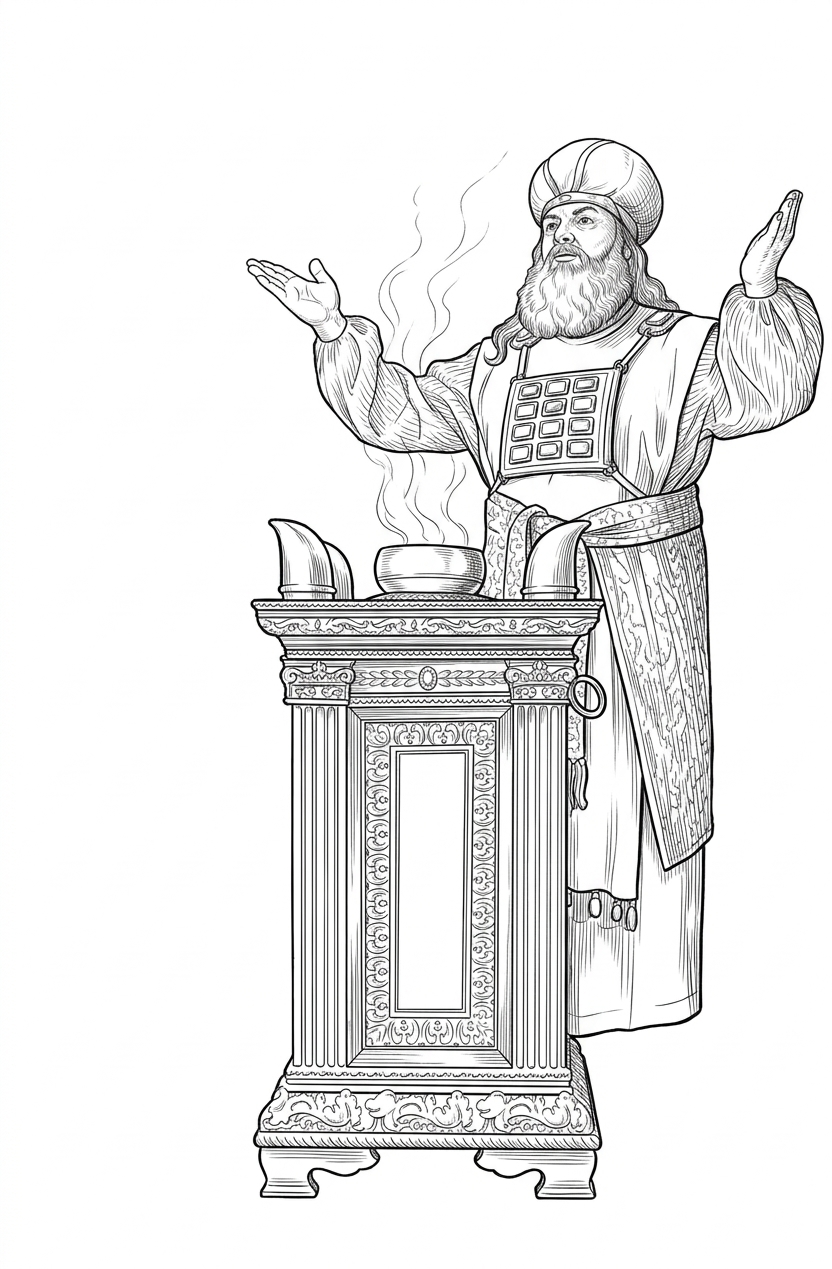
\includegraphics[
    width=0.4\textwidth,
    trim=0 0 0 0,
    clip]{images/golden_altar.jpg}
\end{figure}

\begin{ReaderQuestion}
禱告如香升到神面前（8:3–4）對你而言有什麼意義？當你禱告很久卻看不見改變時，你會如何理解「神聽見了我的禱告」？
\end{ReaderQuestion}

\section{第一號}

\begin{ScriptureBox2}{有什麼丟在地上？圈出地和樹被燒了多少，以及什麼全被燒了。}

\item[8:7] 第一位天使吹號、就有雹子與火攙著血丟在地上．地的三分之一和樹的三分之一被燒了、一切的青草也被燒了。

\end{ScriptureBox2}



\begin{figure}[htbp]
    \centering
    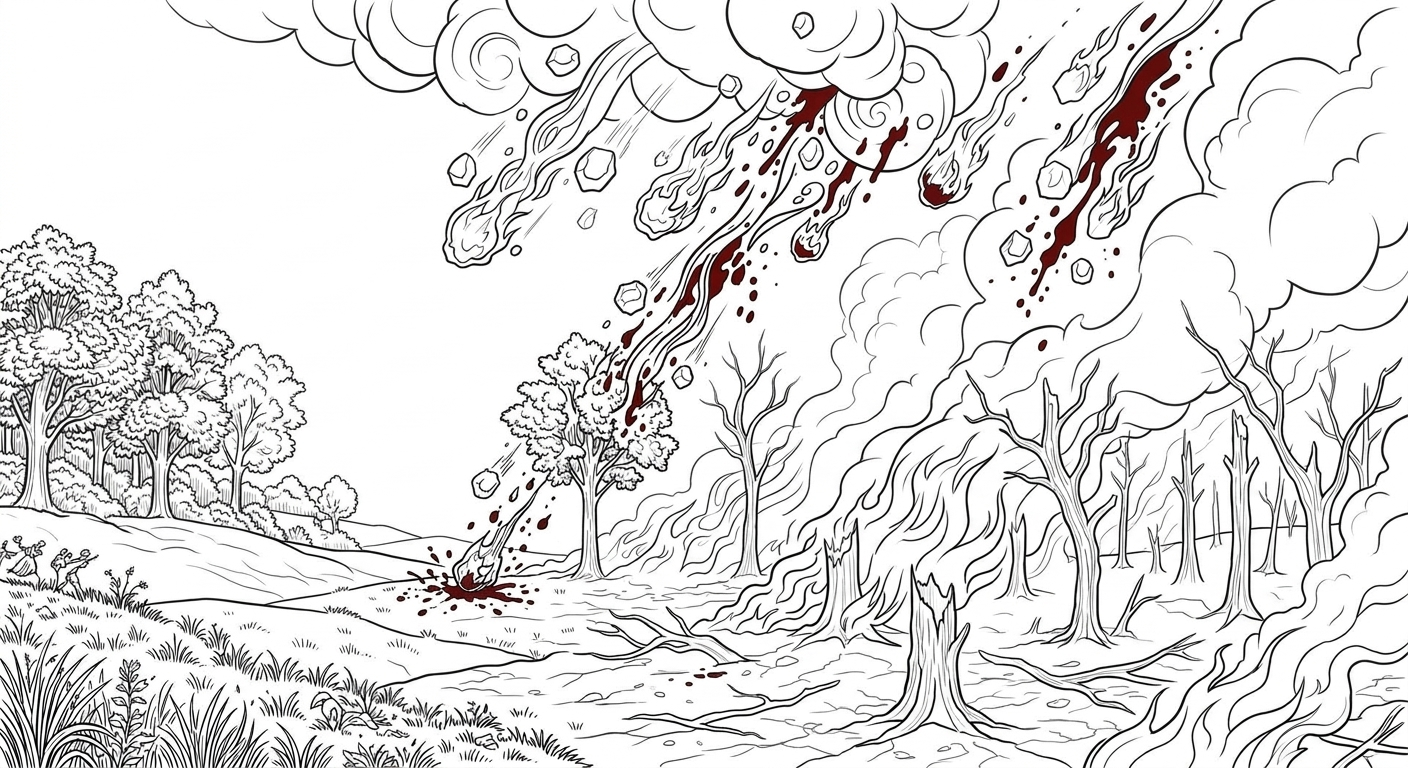
\includegraphics[
    width=1\textwidth, 
    trim=0 0 0 0, 
    clip]{images/trumpet_1st.jpg}
\end{figure}


\section{第二號}

\begin{ScriptureBox2}{數一數8:8–9中「三分之一」出現了幾次。海中有哪三樣受到擊打？}

\item[8:8] 第二位天使吹號、就有彷彿火燒著的大山扔在海中．海的三分之一變成血．

\item[8:9] 海中的活物死了三分之一．船隻也壞了三分之一。

\end{ScriptureBox2}


\begin{figure}[htbp]
    \centering
    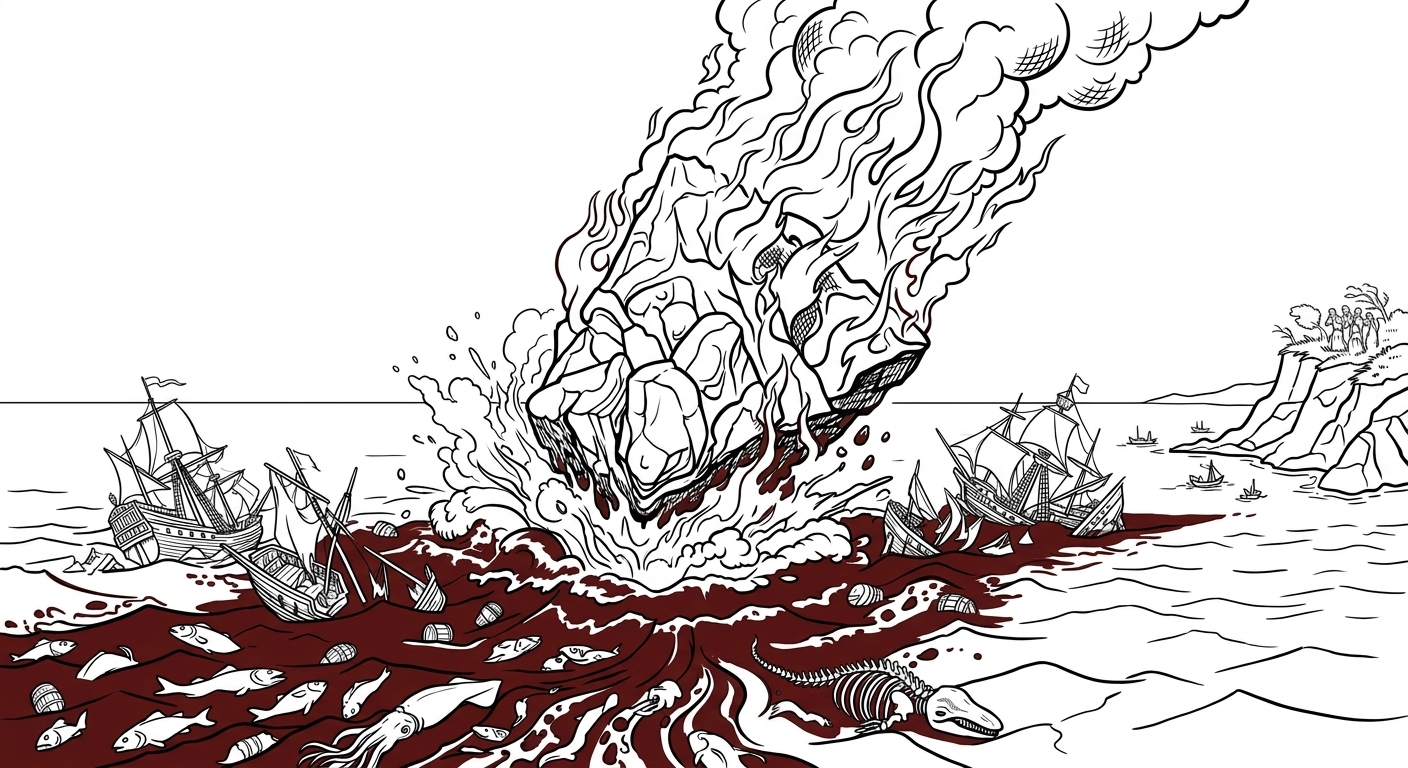
\includegraphics[
    width=1\textwidth, 
    trim=0 0 0 0, 
    clip]{images/trumpet_2nd.jpg}
\end{figure}


\section{第三號}

\begin{ScriptureBox2}{那落下來的星名叫什麼？眾水變成怎樣？喝了那水的人又怎樣？}

\item[8:10] 第三位天使吹號、就有燒著的大星、好像火把從天上落下來、落在江河的三分之一、和眾水的泉源上．

\item[8:11] 這星名叫茵蔯．眾水的三分之一變為茵蔯．因水變苦、就死了許多人。

\end{ScriptureBox2}


\begin{figure}[htbp]
    \centering
    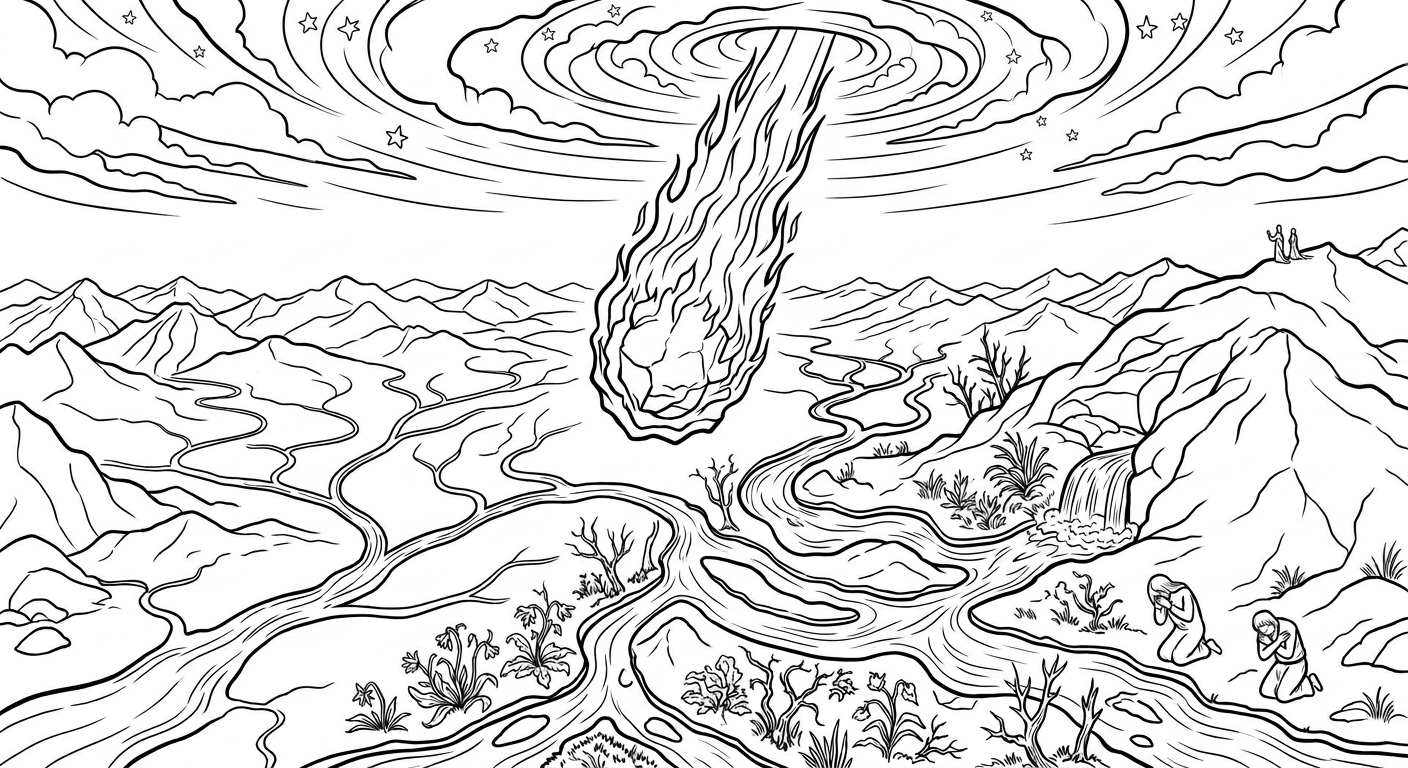
\includegraphics[
    width=1\textwidth, 
    trim=0 0 0 0, 
    clip]{images/trumpet_3rd.jpg}
\end{figure}

「茵蔯\idx{10}{茵蔯}」也叫苦艾、洋艾，希臘文是 apsinthos，英文是wormwood。
這是味道極苦的植物。古代用來驅蟲、入藥，後來也用來製作苦艾酒（absinthe）。
茵蔯在舊約中象徵苦難與審判\idx{15}{審判}。例如耶利米書 9:15說：「我必將茵蔯給這百姓吃，又將苦膽水給他們喝」，以及耶利米哀歌 3:15、阿摩司書 5:7。所以這裡說眾水變為茵蔯，重點在於水變苦、不能喝，帶來死亡。

\section{第四號}

\begin{ScriptureBox2}{天上哪些光體被擊打？各被擊打了多少？白晝和黑夜變成怎樣？}

\item[8:12] 第四位天使吹號、日頭的三分之一、月亮的三分之一、星辰的三分之一、都被擊打．以致日月星的三分之一黑暗了、白晝的三分之一沒有光、黑夜也是這樣。

\end{ScriptureBox2}


\begin{figure}[htbp]
    \centering
    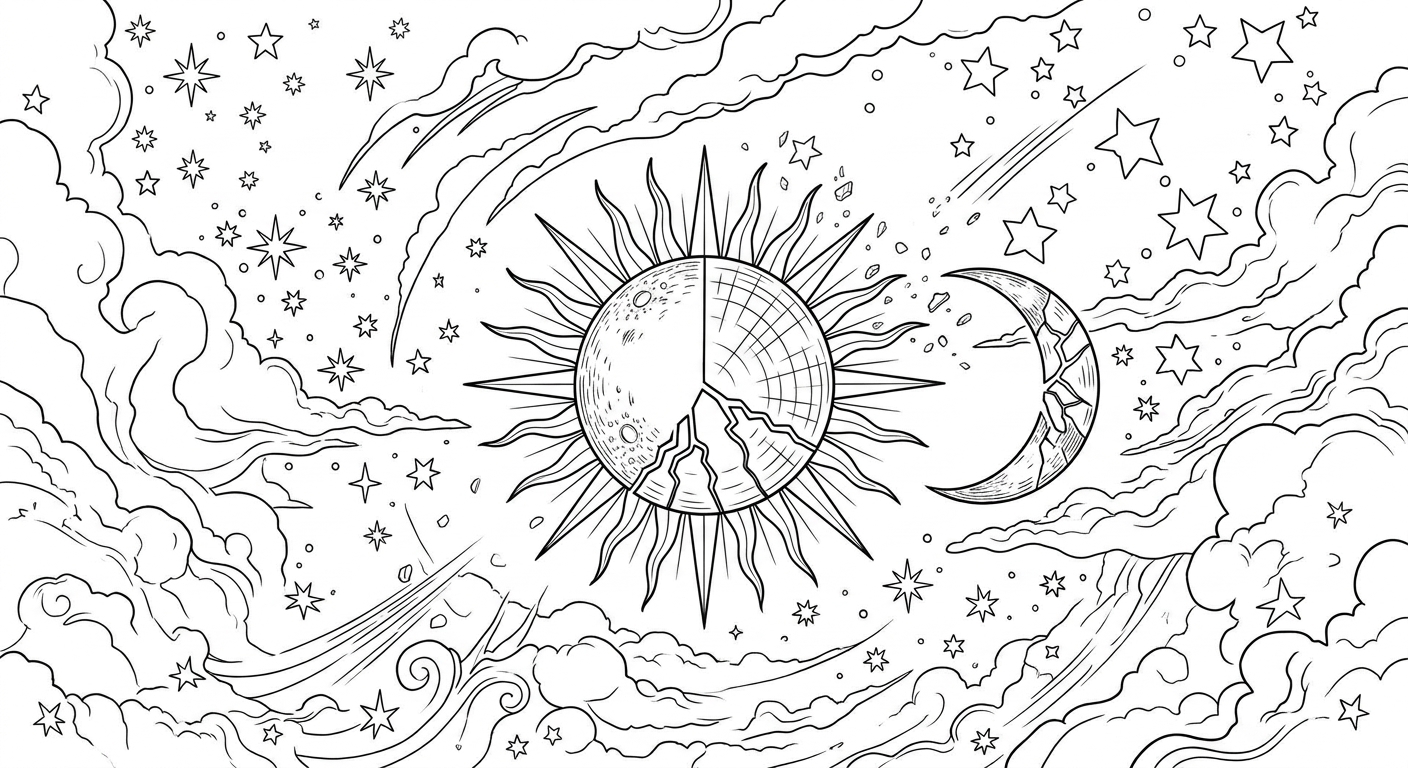
\includegraphics[
    width=1\textwidth, 
    trim=0 0 0 0, 
    clip]{images/trumpet_4th.jpg}
\end{figure}


\section{第五號}

\begin{ScriptureBox2}{在約翰對蝗蟲的描述中，圈出每一個「好像」和「像」。蝗蟲可以傷害誰？牠們又被禁止做什麼？}

\item[8:13] 我又看見一個鷹飛在空中、並聽見他大聲說、三位天使要吹那其餘的號、你們住在地上的民、禍哉、禍哉、禍哉。

\item[9:1] 第五位天使吹號、我就看見一個星從天落到地上．有無底坑的鑰匙賜給他。

\item[9:2] 他開了無底坑、便有煙從坑裡往上冒、好像大火爐的煙．日頭和天空、都因這煙昏暗了。

\item[9:3] 有蝗蟲從煙中出來飛到地上．有能力賜給他們、好像地上蠍子的能力一樣。

\item[9:4] 並且吩咐他們說、不可傷害地上的草、和各樣青物、並一切樹木、惟獨要傷害額上沒有　神印記的人。

\item[9:5] 但不許蝗蟲害死他們、只叫他們受痛苦五個月．這痛苦就像蠍子螫人的痛苦一樣。

\item[9:6] 在那些日子、人要求死、決不得死．願意死、死卻遠避他們。

\item[9:7] 蝗蟲的形狀、好像預備出戰的馬一樣、頭上戴的好像金冠冕、臉面好像男人的臉面。

\item[9:8] 頭髮像女人的頭髮、牙齒像獅子的牙齒。

\item[9:9] 胸前有甲、好像鐵甲．他們翅膀的聲音、好像許多車馬奔跑上陣的聲音。

\item[9:10] 有尾巴像蠍子．尾巴上的毒鉤能傷人五個月。

\item[9:11] 有無底坑的使者作他們的王．按著希伯來話、名叫亞巴頓、希利尼話、名叫亞玻倫。

\item[9:12] 第一樣災禍過去了、還有兩樣災禍要來。

\end{ScriptureBox2}


\begin{figure}[htbp]
    \centering
    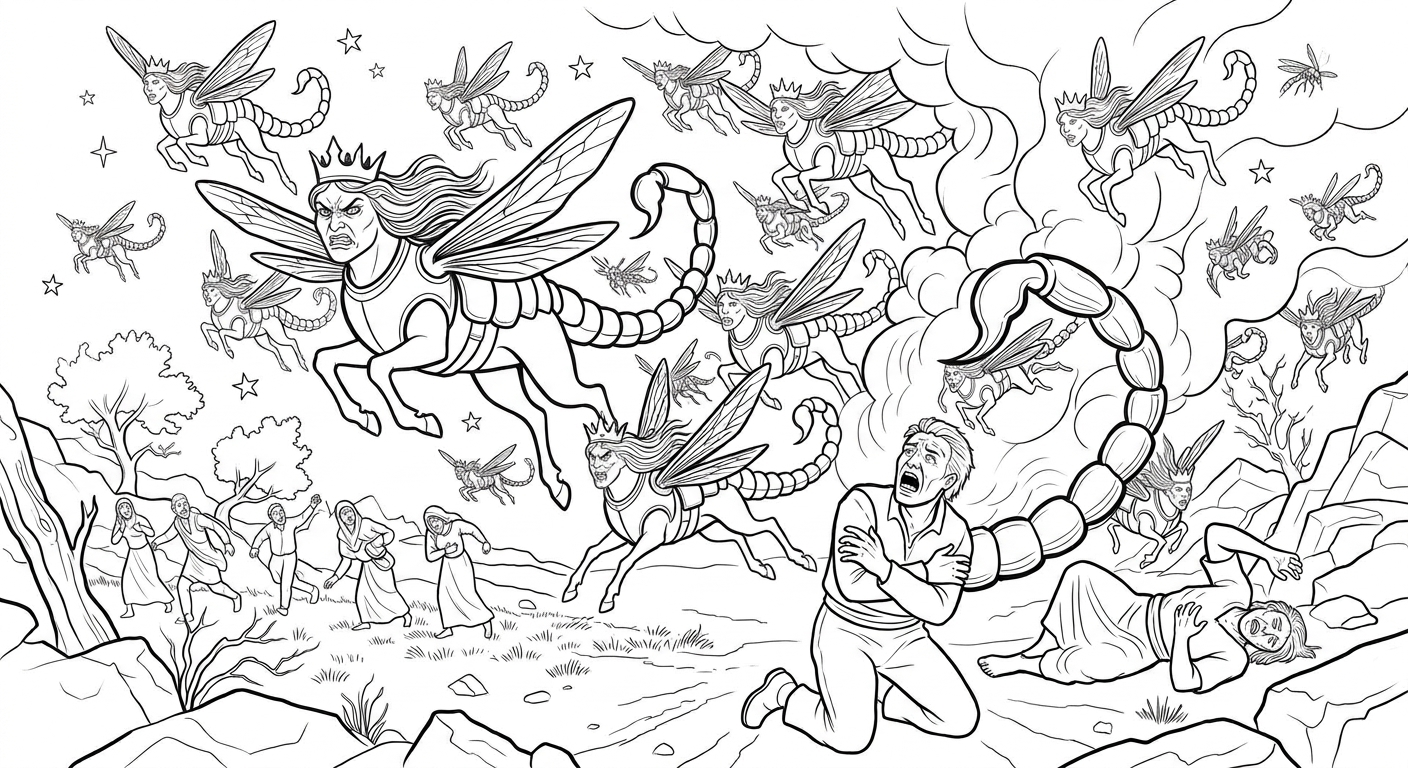
\includegraphics[
    width=1\textwidth, 
    trim=0 0 0 0, 
    clip]{images/trumpet_5th.jpg}
\end{figure}


\section{第六號}

\begin{ScriptureBox2}{9:13的聲音從哪裡出來？將它與8:3比較。然後劃出9:20–21中，那些沒有被殺的人仍然不肯悔改的一切事。}

\item[9:13] 第六位天使吹號、我就聽見有聲音、從　神面前金壇的四角出來、

\item[9:14] 吩咐那吹號的第六位天使、說、把那捆綁在伯拉大河的四個使者釋放了。

\item[9:15] 那四個使者就被釋放．他們原是預備好了、到某年某月某日某時、要殺人的三分之一。

\item[9:16] 馬軍有二萬萬．他們的數目我聽見了。

\item[9:17] 我在異象中看見那些馬和騎馬的、騎馬的胸前有甲如火、與紫瑪瑙、並硫磺．馬的頭好像獅子頭、有火、有煙、有硫磺、從馬的口中出來。

\item[9:18] 口中所出來的火、與煙、並硫磺、這三樣災殺了人的三分之一。

\item[9:19] 這馬的能力、是在口裡、和尾巴上．因這尾巴像蛇、並且有頭用以害人。

\item[9:20] 其餘未曾被這些災所殺的人、仍舊不悔改自己手所作的、還是去拜鬼魔、和那些不能看、不能聽、不能走、金、銀、銅、木、石、的偶像。

\item[9:21] 又不悔改他們那些凶殺、邪術、姦淫、偷竊的事。

\end{ScriptureBox2}


\begin{figure}[htbp]
    \centering
    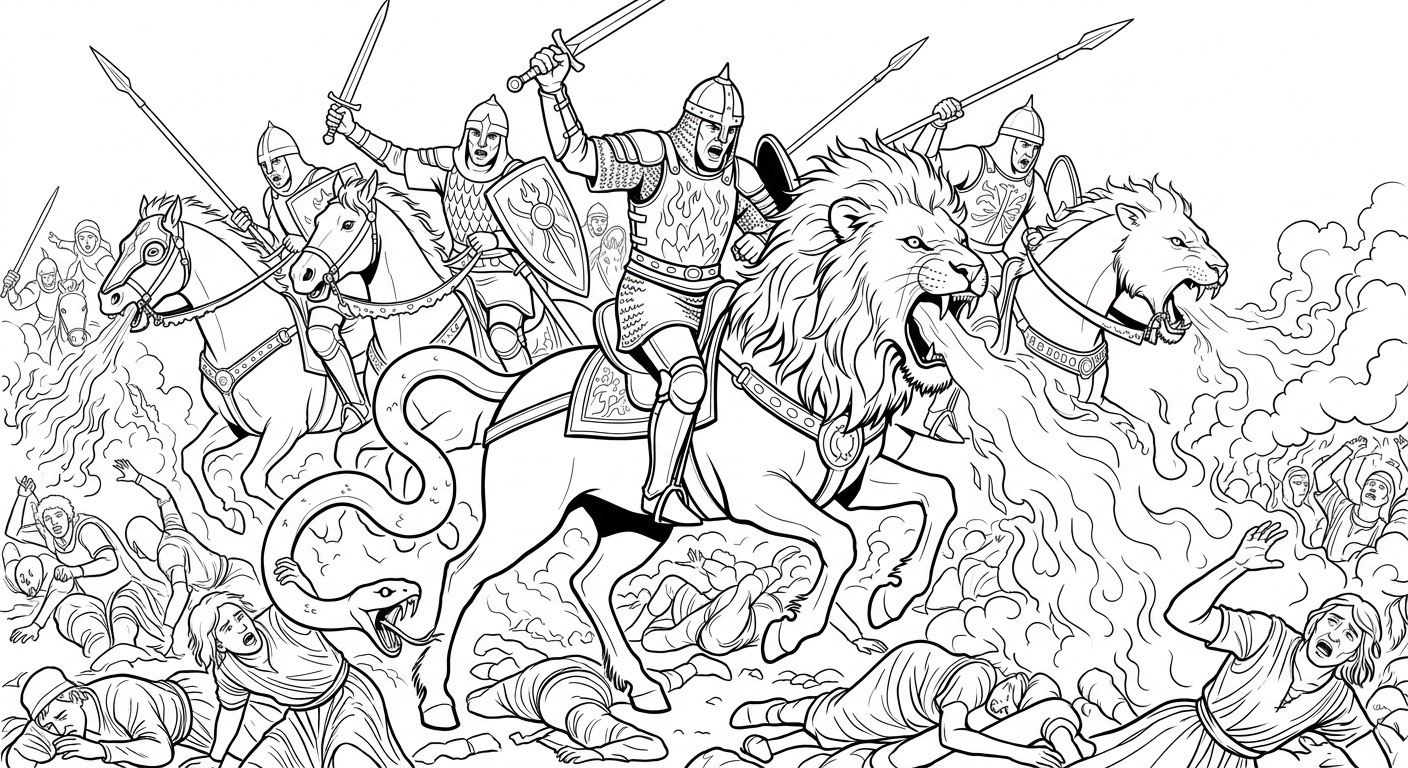
\includegraphics[
    width=1\textwidth, 
    trim=0 0 0 0, 
    clip]{images/trumpet_6th.jpg}
\end{figure}

「那捆綁在伯拉大河\idx{07}{伯拉大河}的四個使者」現在被放出來，執行任務。他們可能是被捆綁的墮落天使或邪靈，或是歷史上的軍事勢力。他們組織了二萬萬的馬軍，是要殺死人類的三分之一。
「馬軍有二萬萬」希臘文直譯是「萬萬的萬萬」，即數量極大的軍隊。所以不一定是 20,000 乘以 20,000 等於 400,000,000。

「伯拉大河」（Euphrates）不僅是以色列\idx{05}{以色列}東北方的重要地理界線，也與神所應許的疆界，以及從東北方而來的外敵和審判\idx{15}{審判}有關。\footnote{例如，神與亞伯拉罕立約時，應許將從埃及河直到伯拉大河一帶的土地賜給他的後裔（創世記 15:18）。另一方面，以賽亞書以伯拉大河水勢洶湧、氾濫溢出的景象，比喻亞述王及其軍隊的勢力，並描寫這股勢力如洪水般臨到猶大（以賽亞書 8:7–8）。} 在這裡，這場審判的範圍已超越古代以色列的疆界，涉及全人類。

這麼大的災禍應該是帶來悔改\idx{10}{悔改}吧？可是災難不能取代悔改。這裡讓我們了解人最大的危機是拒絕悔改。

\begin{ReaderQuestion}
9:20–21特別指出，人經歷災禍之後仍然「不悔改」。為什麼苦難與災難不一定使人悔改？這段經文對我們今天理解「悔改」有什麼提醒？
\end{ReaderQuestion}

值得注意的是，「三分之一」反覆出現。神在七號\idx{02}{七號}中仍然限制。並沒有毀滅整個受造界。


\begin{figure}[htbp]
    \centering
    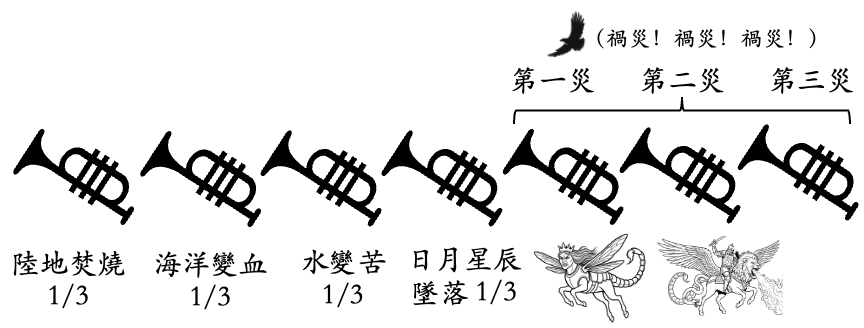
\includegraphics[
    width=1\textwidth, 
    trim=0 0 0 0, 
    clip]{images/trumpets_woes.png}
    \caption{第一號到第七號}
    \label{fig:trumpets_woes}
\end{figure}



\section{未來的事件，古老的語言}

你可能會注意到，神仍讓約翰以馬匹、騎兵和刀劍等第一世紀所熟悉的戰爭武器來描述這些未來事件。可是現在的戰爭已經不使用馬匹和刀劍，而是使用無人機與戰鬥機。以後的戰爭更應該是高度發展的軍事科技。你可能會問，如果啟示錄中的異象確實是未來事件，那麼，為甚麼約翰仍然使用馬匹和刀劍來描述這些異象？神怎麼不直接讓約翰看見並描述未來的軍事科技？甚至可能有人會問，馬是不是坦克？火是不是導彈？蝗蟲\idx{15}{蝗蟲}是不是直升機？

一個比較中肯的答案是，神不是要約翰傳講「未來的武器科技」，而是「神的審判\idx{15}{審判}」。
我們需要了解，看見未來科技未必就是明白神的啟示。神用約翰能傳達的方式給他當時的人以及後來的人。
例如，啟示錄9:7說：「蝗蟲的形狀好像預備出戰的馬。」啟示錄9:17又說「馬的頭好像獅子的頭……」啟示錄9:19則說：「牠們的尾巴好像蛇。」約翰不是說「我看見了馬。」而是不斷使用「好像」的語言來描述他所看見的異象。試想神真的讓約翰看到一架F-35戰機，約翰會怎樣描述？他可能會說：「我看見一隻巨大的鐵鳥，有兩個翅膀，口中吐火，從天上飛過。」啟世錄中大量使用「好像」、「如同」等等，顯示約翰是以他的時代的語言描述所看見的異象。因此，我們如果把啟示錄的敘述直接轉換成阿帕契（Apache）直升機、現代坦克等，並不是好的解經方法。\footnote{Beale, G. K. (1999). Bauckham, R. (1993).}

我們再舉一個例子。例如啟示錄9章的「蝗蟲像戰馬」幾乎明顯對應約珥書中預言關於末世的審判的場景「牠們的形狀如馬，奔跑如馬兵。」（約珥書2:4）
收到約翰書信的讀者就會聯想到約珥書的「 耶和華的日子」「審判 」「末世」。因此神若讓約翰看到一架「F-35」，反而可能破壞了其中跟舊約的關係。
